\section{Fjernbetjening}

For at øge sikkerheden er det besluttet at koble en fjernbetjening til dronen. Fjernbetjeningen skal udelukkende bruges til at overtage styring af dronen, hvis noget skulle gå galt. For at kunne finde den bedst egnede fjernbetjening til projektet, er der opstillet nogle kriterier:

\begin{itemize}
	\item Antal kanaler.
	\item Pris.
	\item Rækkevidde.
\end{itemize}

Som udgangs punkt skal fjernbetjeningen minimum have 4 kanaler, disse skal bruges til styringen af dronen. Udover de 4 kanaler, ønskes en yderligere kanal. Denne kanal skal bruges til at tilkoble/afbryde den autonome del af dronen. Dette betyder at der ønskes en fjernbetjening med minimum 5 kanaler, helst fordelt som på figur~\ref{fig:fjernbetjening} 

\begin{figure}[H]
\centering
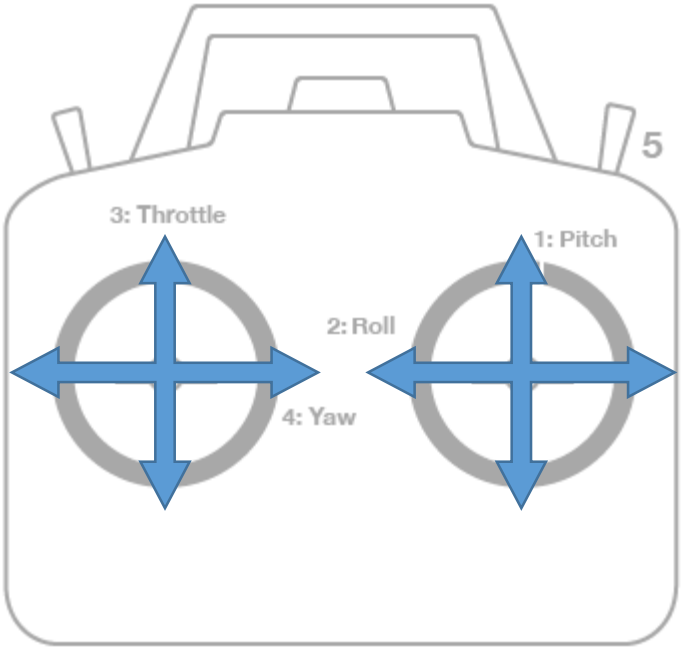
\includegraphics[width=0.5\textwidth]{Billeder/Fjernbetjening}
\caption{Fjernbetjening}
\label{fig:fjernbetjening}
\end{figure}

Hvor 4 af kanalerne bruges til selve styringen (Pitch, Roll, Throtte \& Yaw). Med disse kanaler er det muligt at få fuld kontrol over dronen.
Da fjernbetjeningen ikke har den største funktionalitet i systemet, ønskes det at finde en billig løsning. 

Da det ønskes at drone skal flyve autonomt over større områder er det nødvendigt med en stort rækkevidde på fjernbetjeneren.  

Ud fra valget af drone og erfaringer fra andre brugere, blev det besluttet at købe en Spektrum DX5e 5 kanals fjernbetjening.